%Architecture

Reliability is being explored at different layers of abstraction; from devices~\cite{Datta2014,Datta2015,Rahul2015} to memory~\cite{isca2014} to algorithms.
At a circuit-level, ~\cite{chen2015fast} uses a conditional probability approach for modeling reliability in combinational circuits.

In this section, we evaluate the capabilities of a popular visual object recognition algorithm - HMAX - and exploit the potential to save 
power and reduce computational load.

\subsection{Power}
Many previous works have looked at tackling the increasing refresh power in DRAMs~\cite{Liu2012, Stuecheli2010}. In ~\cite{Liu2011}, the 
authors looked at reducing refresh power on multimedia workloads. Recently, in ~\cite{iccd2014}, the authors showed that in 
real-time embedded vision applications, refresh power can dynamically be changed based on autonomously tagging data with logical labels.

HMAX is a hierarchical visual object recognition model that has been used in various embedded real-time applications~\cite{Kestur2012, Maashri2012a}. In this work, we explore the resiliency of HMAX to bit errors that can then be used to choose the refresh rate for DRAMs when these images are stored.  
Fig.~\ref{fig:hmax_pixel_sensitivity} illustrates the classification accuracy of HMAX as a function of the pixel errors introduced in each image.

%HMAX Resilience
\begin{figure}[htb!]
\vspace{0pt}
\centering
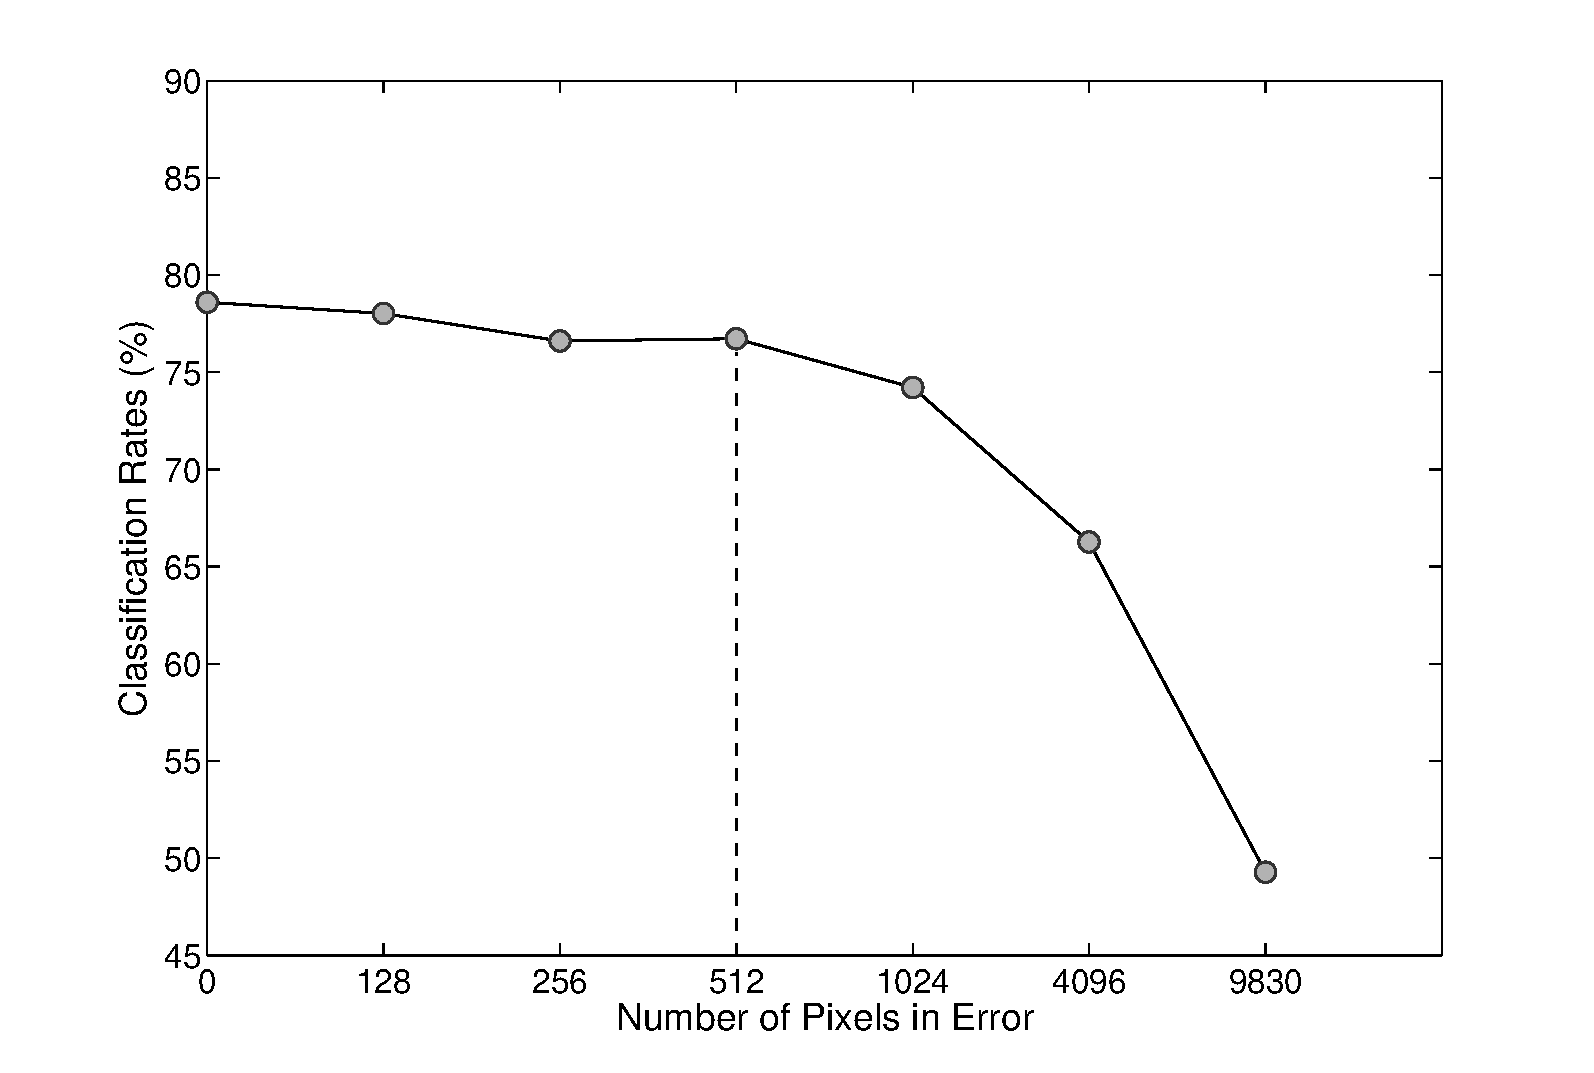
\includegraphics[width=0.99\linewidth,trim={20 20 30 20}, clip]{./figures/PixelSensitivityAnalysis.pdf}
\vspace{0pt}
\caption{HMAX resilience to errors. Six classes from CalTech101 were used.}\label{fig:hmax_pixel_sensitivity}
\vspace{0pt}
\end{figure}

\subsection{Compute}
In this section we explore the potential savings in computational work needed to be done while not compromising on accuracy. The input image 
is passed through an image pyramid before computing the ``S1'' layer of HMAX. The original HMAX model uses a bicubic interpolation technique 
to generate the image pyramid. In the embedded version, compute resources are very costly. Saving a few resources can result in being able to 
fit a design in a particular form-factor or may cause the design to overflow into the next larger generation of devices. We explored the 
capablity of HMAX to correctly recognize objects using bilinear interpolation in the image pyramid. The impact of this is that instead of 
44 multipliers (bicubic interpolation), we would need just eight multipliers (bilinear interpolation). Table~\ref{table:compute} shows the 
results. 

\begin{table}[h]
\renewcommand{\arraystretch}{1.3}
\caption {Interpolation Tecniques}
\label{table:compute}
\begin{tabular}{lllll}
 System & Algorithm & Accuracy & Resources\\\hline
 HMAX	& Bicubic   & 54\% & 44\\\hline
 HMAX   & Bilinear  & 53\% & 8\\\hline
\end{tabular}
\end{table}
